\section{Phasendiagramm eines 2DES}
\label{sec:theo_phasendiagramm}

Das Phasendiagramm eines 2DES auf flüssigem Helium wird bestimmt durch das Wechselspiel folgender Energien:
\begin{itemize}
	\item thermische Energie $E_\text{therm}=k_\text{B}T \propto T\quad$\phantom{$\frac{\hbar^2}{\epsilon_0}$}
	\item Coulomb"=Energie $E_\text{Coulomb}=\frac1{4\pi\epsilon_0} e^2\sqrt{\pi n} \propto \sqrt{n}\quad$\phantom{$\frac{\hbar^2}{\epsilon_0}$}
	\item Fermi"=Energie $E_\text{F}=\frac{\pi\hbar^2}{m_e}n\propto n$
\end{itemize}
Diese sind abhängig von den thermodynamischen Parametern des Systems. Wie aus obiger Aufstellung ersichtlich ist, sind dies die Elektronendichte $n_s$ und die Temperatur $T$ des Elektronensystems. $n_s$ und $T$ sind die im Phasendiagramm interessanten Achsen; zusätzlich sind das Magnetfeld $B$ und auf dünnen Heliumfilmen die Polarisierbarkeit des Substrats weitere Parameter, die das Phasenverhalten des 2DES modifizieren. Diese können als weitere Achsen des Phasendiagramms dienen.

Bei typischen Elektronendichten von $10^{9}$ bis $\unit[10^{13}]{\Em}$ verhalten sich die Elektronen klassisch, da die Fermi"=Energie im Bereich von $0.003$ bis $\unit[30]{mK}$ liegt. Das bedeutet, dass die Fermi"=Energie bei Experimenten mit 2DES auf Bulk"=Helium im hier erreichbaren Temperaturbereich keine Rolle spielt. Deshalb ist hier das Verhältnis der Größen der thermischen Energie und der Coulomb"=Energie wichtig. Dies kann zum Phasenübergang vom klassischen Elektronengas zum Elektronenfestkörper, dem so genannten Wigner-Kristall führen. Dieses Phänomen wurde theoretisch von \name{E.~Wigner} \cite{Wig34} vorhergesagt.

Wenn man in der Lage ist, wie für Elektronen auf dünnen Heliumfilmen theoretisch vorhergesagt, die Elektronendichten in Bereiche bis zu \unit[10$^{16}$]{\Em}  zu erhöhen, dann wird das Verhältnis von Fermienergie und Coulomb"=Energie bestimmend für den Zustand des Systems. Man nähert sich einem weiteren Phasenübergang vom Wigner"=Kristall zum Zustand des entarteten Fermi-Gases von Elektronen, welcher schon aus der Physik von Elektronen in Halbleitern und Metallen bekannt ist.

\subsection{Übergang zum Elektronenfestkörper nach \name{Wigner}}

Wie \name{E.~Wigner} bereits in \cite{Wig34} bei der Untersuchung der Wechselwirkung von Elektronen in Metallen festgestellt hat, können die Elektronen mit einer kompensierenden positiven Ladung im Hintergrund und bei geringer kinetischer Energie in drei Dimensionen einen $bcc$-Kristall bilden. Dies passiert, obwohl ihre Wechselwirkung durch die Coulomb-Kräfte rein abstoßend ist. Einen solchen Übergang kann man auch in zwei Dimensionen beobachten, was von \name{R.~Crandall} \ea{} \cite{Cra71} für das System von Elektronen auf Helium und von \name{A.~Chaplik} \ea{} \cite{Cha72} für Elektronen oder Löcher in Halbleiter-Inversionsschichten vorgeschlagen wurde. Der erste experimentelle Nachweis dieses Phasenübergangs bei Elektronen auf Bulk"=Helium gelang \name{Grimes} und \name{Adams} \cite{Gri79}.

Den Phasenübergang von der klassischen Elektronenflüssigkeit zum Elektronenfestkörper erwartet man, wenn die potentielle Energie $\brak{V}$ der Elektronen über ihre thermische Energie $\brak{K}$ dominiert. Der Parameter $\Gamma$ steht für das Verhältnis dieser beiden Größen und charakterisiert das thermodynamische Verhalten des Systems bezüglich des Phasenübergangs:
    \begin{equation}
        \label{eqn:tph_VWRatio}
        \frac{\brak{V}}{\brak{K}} \equiv \Gamma\quad.
    \end{equation}
Für ein klassisches 2DES ist
	\begin{equation}
		\label{eqn:Gamma_klass}
		\Gamma=\frac1{4\pi\epsilon_0}\frac{e^2\sqrt{\pi n}}{\kB T}\quad.
	\end{equation}
Der Wert von $\Gamma$ bestimmt das thermodynamische Verhalten des 2DES im Bezug auf die Wigner-Kristallisation:
\begin{description}
	\item[$\Gamma\lesssim1$:] In diesem Bereich dominiert die kinetische Energie der Elektronen. Es liegt ein klassisches Elektronengas vor. Die Fermi-Energie ist bei den üblichen Elektronendichten im Bereich einiger Millikelvin und spielt daher hier keine Rolle.
	\item[$1\lesssim\Gamma\lesssim100$:] In diesem Bereich wird die Elektronenbewegung hochkorreliert, allerdings findet noch keine Kristallisation statt.
	\item[$\Gamma\gtrsim100$:] Hier dominiert die potentielle Energie. Man erwartet einen Phasenübergang, nach dem die Elektronen in einem periodischem Gitter angeordnet sind.
\end{description}

Der Phasenübergang vom Wigner"=Kristall zur klassischen Elektronenflüssigkeit  wird von der \mbox{KTHNY}\footnote{Kosterlitz und Thouless \cite{Kos73}, Nelson und Halperin \cite{Nel79} und Young \cite{You79}}-Theorie gut beschrieben. Diese Theorie beinhaltet, dass der Vorgang des Schmelzens durch das Aufbrechen vorher gebundener Paare von Versetzungen im Kristallgitter initiiert wird.

Eine molekulardynamische Simulation von \name{R. Morf} \cite{Mor79} auf Basis der KTHNY"=Theorie ergab einen Bereich von $125<\Gamma<132$. Für ein 2DES auf dünnen Heliumfilmen bestimmten \name{F.~Peeters} \ea{} \cite{Pee83} mit Hilfe numerischer Simulationen und einem Wert von $\Gamma(d=\infty)=137$ das in Abbildung~\ref{fig:phase_diag_scheme} zu sehende Phasendiagramm für Elektronen auf Bulk"=Helium und dünnen Heliumfilmen auf metallischen und dielektrischen Substraten. 

\begin{figure}[h!tbp]
	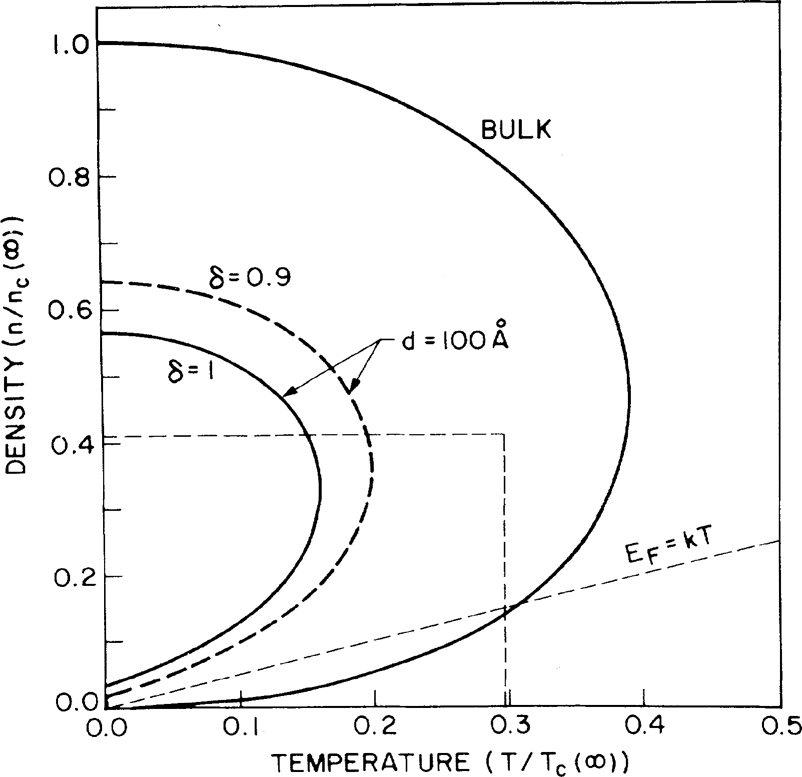
\includegraphics[width=\smallwidth]{theo_phasendiagramm/Pee83_PD}%
	\hfill%
	\begin{minipage}[b]{\textwidth-\smallwidth-\tabcolsep}
	\caption[Schematisches Phasendiagramm des 2DES.]{Schematisches Phasendiagramm des 2DES nach \cite{Pee83}. Zusätzlich zur Phasengrenze auf Bulk"=Helium ist hier noch der Verlauf auf einem \unit[10]{nm} dünnen Heliumfilm auf Saphir ($\delta=0.9$) und metallischem Substrat ($\delta=1$) angezeigt.\par$n_c=\unit[2.4\times10^{16}]{\Em}$ und $T_c=\unit[33]{K}$.}
	\label{fig:phase_diag_scheme}
	\end{minipage}
\end{figure}

\subsubsection{Phasendiagramm auf dünnen Heliumfilmen}
\label{ssec:phasediag_films}
Weil auf dünnen Heliumfilmen der Charakter der Elektron"=Elektron ($e$-$e$) Wechselwirkung stark von der Elektronendichte und der Helium-Filmdicke abhängig ist, bleibt auch das Phasendiagramm des 2DES davon nicht unberührt. In Abbildung~\ref{fig:phase_diag_scheme} sieht man, dass der Bereich des Wigner"=Kristalls im Phasendiagramm auf dünnen Heliumfilmen dadurch deutlich reduziert wird. Maximal wird dieser Effekt für ein metallisches Substrat ($\delta=1$).
\enlargethispage{2ex}

Nach den analytischen Rechnungen von \name{M.~Saitoh} \cite{Sai89} und dem Vergleich mit Messungen von \name{A.~Dahm} wurde für $\Gamma(d)\approx137$ auf dünnen Heliumfilmen ein ähnlicher Wert wie für Bulk"=Helium bestimmt. Nach \name{Saitoh} gilt für die Schmelztemperatur $T_m(d)$ näherungsweise
\begin{equation}
	\label{eqn:wc_melting_temp}
	k_BT_m(d)=\frac1{4\pi\epsilon_0}\frac{e^2\sqrt{\pi n}f(d)}{\Gamma(d)}\ttextt{mit}
	f(d)=1-\delta\left(1+4\pi n \frac{d^2}{c_0^2}\right)^{-\frac32}\quad.
\end{equation}
Hierbei ist $\delta=(\epsilon_{r,\text{Substrat}}-1)/(\epsilon_{r,\text{Substrat}}+1)$ und $c_0=1.1061$ eine Konstante. Diese Formel wird später im Abschnitt~\ref{ssec:wigner_auswertung} bei der Berechnung der $\Gamma$-Werte der Phasenübergänge Verwendung finden.

\subsection{Übergang vom Elektronenfestkörper zum entarteten Fermi"=Gas}
Beim Übergang vom Elektronenfestkörper zum entarteten Fermi"=Gas ist es das Wechselspiel zwischen Coulomb"=Energie und Fermi"=Energie, das den Phasenübergang bestimmt:
\begin{equation}
	\label{eqn:qm_Gamma}
	\Gamma_\text{QM}=\frac{E_\text{Coulomb}}{E_\text{Fermi}}
		=\frac{m_e e^2}{4\pi\epsilon_0\hbar^2 \sqrt{\pi}}\frac1{\sqrt{n}}\quad.
\end{equation}
Die Ordnung des 2DES im Wigner"=Kristall, hervorgerufen durch die über die thermische Energie des Systems dominierende Coulombenergie, wird aufgrund der bei hohen Elektronendichten starken Einschränkung der Elektronen im Ortsraum wieder zerstört. Aufgrund der Heisenbergschen Unschärferelation nehmen dann die Fluktuationen der Elektronen im Impulsraum stark zu. Dies hat zur Folge, dass der Wigner"=Kristall schmilzt und man ein entartetes Fermi"=Gas erhält.

